\documentclass[11pt, a4paper]{article}

\usepackage[utf8x]{inputenc}
\usepackage[spanish]{babel}
\usepackage[linktoc=all]{hyperref}
\usepackage{multicol}

\usepackage{graphicx}
\usepackage{float}

\usepackage{listings}
\usepackage{xcolor}
 
\definecolor{codegreen}{rgb}{0,0.6,0}
\definecolor{codegray}{rgb}{0.5,0.5,0.5}
\definecolor{codepurple}{rgb}{0.58,0,0.82}
\definecolor{backcolour}{rgb}{0.95,0.95,0.92}
 
\lstdefinestyle{mystyle}{
    backgroundcolor=\color{backcolour},   
    commentstyle=\color{codegreen},
    keywordstyle=\color{magenta},
    numberstyle=\tiny\color{codegray},
    stringstyle=\color{codepurple},
    basicstyle=\ttfamily\footnotesize,
    breakatwhitespace=false,         
    breaklines=true,                 
    captionpos=b,                    
    keepspaces=true,                 
    numbersep=5pt,                  
    showspaces=false,                
    showstringspaces=false,
    showtabs=false,                  
    tabsize=2
}

\lstset{style=mystyle}

%------------------- Dimensiones -------------------
\usepackage{geometry}
\geometry{a4paper,total={170mm,257mm},left=15mm,right=15mm,top=20mm,}
%----------------------------------------------------


\usepackage{fancyhdr}
%------------------- Encabezado y Pie de pág -------------------
\pagestyle{fancy}
\fancyhf{}
\lhead{Tecnicas Digitales II}
\rhead{Trabajo práctico final}
\rfoot{Página \thepage}
%-------------------------------------------------------------	

\begin{document}
\begin{titlepage}
 \centering
	
\includegraphics[scale=0.80]{Imagenes/LOGO.jpg} \par
 	\vspace{1cm}
 	{\scshape\LARGE Universidad Tecnológica Nacional \par}
 	{\scshape\large Facultad Regional de Córdoba \par}
 	\vspace{1cm}
	{\bfseries \Large Trabajo Práctico Final \par}
	{\bfseries \Large Secuencia de leds sobre RaspberryPi \par}
 	\vspace{1.5cm}

	\begin{tabular}{ll}
		Navarro, Facundo			&	63809 	\\
		Nobile, Jonathan Bleddyn	&	69325	
	\end{tabular}
	
	\vspace{1cm}
	Curso: 4R2 \\
	Grupo $N^{\circ} 13$
 	\vfill
	{\bfseries \Large Técnicas Digitales II\par}

	\vspace{1.5cm}
	Docentes: \par
	Ing. Perez Paina, Gonzalo\par
	Ing. Pereyra, Estefanía \par

 	\vfill
	{\large \today\par}
\end{titlepage}
%---------------------------------------------------------------	
	
%--------------------- Indice ----------------------------------	
\tableofcontents
\clearpage
%---------------------------------------------------------------	

\section{Introducción}

Este proyecto consiste en integrar dichos ejercicios de la siguiente manera:
\begin{itemize}
	\item Realice un programa a fin de que el usuario pueda seleccionar desde un menú, una de ocho secuencias de luces posibles. Cuatro de ellas serán comunes para todos los proyectos y son: `` El auto fantástico", ``El choque", ``La apilada" y ``La carrera". Los otros cuatros serán propios de cada grupo y se deberán implementar dos de ellas con algoritmo y los dos restantes por medio de la técnica de tablas de datos.
  \item Implemente el control de acceso a este menú mediante password.
  \item Cada vez que el usuario seleccione una secuencia el programa deberá cambiar la pantalla para indicar cual secuencial está ejecutándose y cómo hacer para salir de la misma. Al optar por abandonar la actual, el programa deberá regresar al menú principal inmediatamente sin completar la secuencia que se está desarrollando y apagando todas las luces.
  \item Permita la posibilidad de controlar la velocidad de cada secuencia. Presionando la flecha hacia arriba se incrementará la velocidad y presionando la flecha hacia abajo se reducirá. Introduzca el censado de las teclas oprimidas en el lugar apropiado de su programa a fin de percibir la reacción del sistema en forma inmediata, independiente de la velocidad actual. La velocidad ajustada en cada secuencia deberá conservarse entre llamadas a diferentes secuencias.
  \item El valor inicial correspondiente a la velocidad de las secuencias deberá ingresarse mediante la lectura del estado de los potenciómetros que están conectados a las entradas analógicas del conversor A/D.
  
  \item Generar una opción en el programa que permita establecer dos modos de trabajo: local y remoto. En modo local las secuencias de luces se ejecutarán en los leds que se encuentran en el hardware adicionado a la placa Raspberry donde se ejecuta el programa. En modo remoto las secuencias se ejecutarán sobre el hardware adicional colocado en otra Raspberry y conectada a la que ejecuta el programa mediante un cable serie RS-232. Se podrá usar el mismo programa para implementar esta opción en las dos Raspberry o realizar uno principal y otro secundario.
  \item Como opción genere una sección destinada a establecer las velocidades iniciales de las secuencias realizando el ajuste de los potenciómetros.
\end{itemize}

\section{Objetivos}
Aplicar los conceptos aplicados durante el transcurso de la materia, aglutinar los puntos prácticos en un solo programa sobre la placa de desarrollo RaspberryPi. 

\clearpage %SALTO DE PAGINA


\section{Diagrama de flujo}
EL programa al iniciar, pide una contraseña ya establecida, si la misma se ingresa erróneamente en 3 oportunidades el programa termina, caso contrario se pasa al menú principal.

En este nivel se visualiza un pequeño listado de las secuencias disponibles, valores de velocidad y $ADC$, como así también en un texto titilante se hace hincapié en las teclas para proseguir o finalizar el programa. Dentro del menu principal presionando:

\begin{itemize}
	\item \textbf{Q} : Se finaliza el programa.
	\item \textbf{R}: Se conmuta a \textit{modo remoto}, a través de la comunicación serie. Volviendo a presionar \textbf{R} se vuelve a \textit{modo local}.
	\item \textbf{P} : Se pasa el valor leído del $ADC$ (en porcentual) al valor de la variable ``velocidad".
	\item \textbf{1 ... 8} : Se ingresa a la secuencia seleccionada.
\end{itemize}

Al pasar a alguna de las secuencias seleccionadas se puede modificar el valor de la velocidad  apretando las teclas \textbf{``UP/DOWN"} , para finalizar la secuencia se debe presionar \textbf{Q} y se vuelve al menú principal.
\begin{figure}[H]
	\centering
	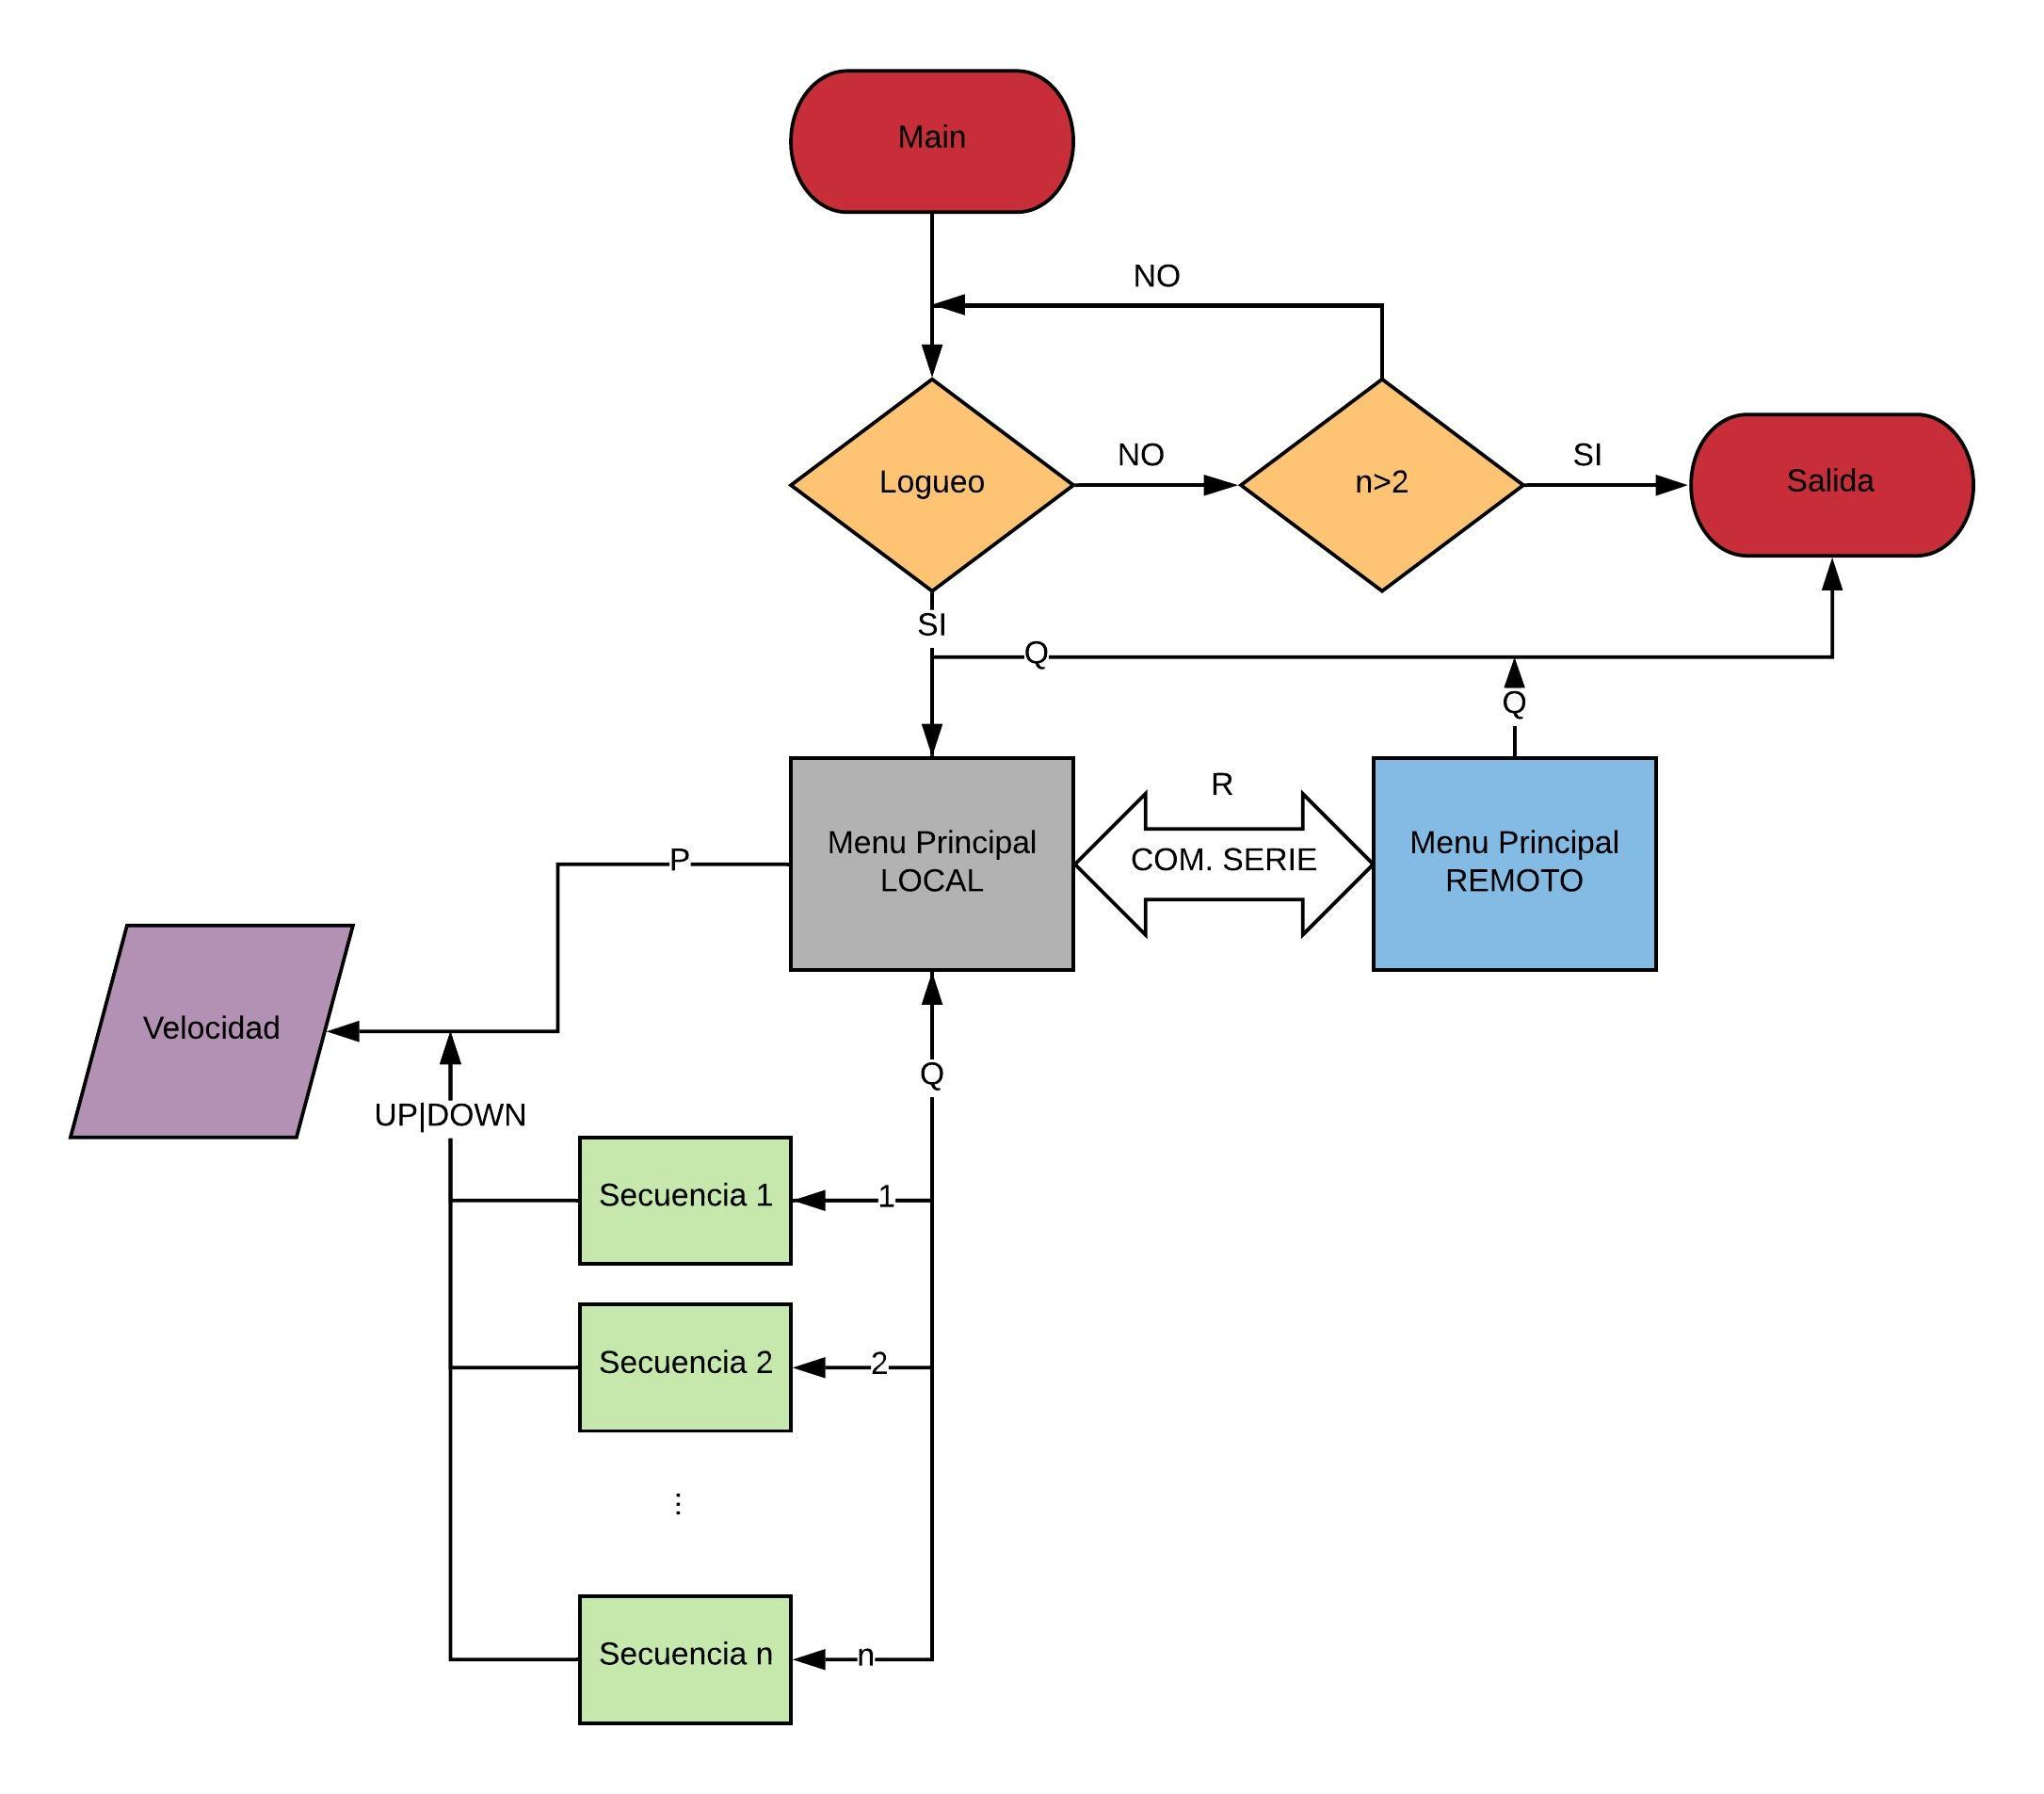
\includegraphics[width = \textwidth]{Imagenes/dflujo.jpg}
	\caption{Diagrama de flujo del programa.}
	\label{dflujo}
\end{figure}


\clearpage %SALTO DE PAGINA

\section {$main.c$}
El archivo fuente $main.c$ contiene la estructura principal del programa, a través del cual se llaman las funciones periféricas. A continuación se explicaran las partes fundamentales.

\subsection{Inicialización de GPIO.}
\lstinputlisting[language=C, firstline=34 , lastline=34, caption =Fragmento de main.c ]{code/main.c}
\lstinputlisting[language=C, caption = led\_config.c]{code/led_config.c}
A penas se ingresa al programa se inicializa la configuración de los GPIO para que se comporten como salida, los mismos corresponden a los leds. 
\\

\subsection{nCurses inicialización}

\lstinputlisting[language=C, firstline=35 , lastline=44, caption =Fragmento de main.c ]{code/main.c}

\subsection{Inicialización de ADC y captura de datos.}

\lstinputlisting[language=C, firstline=45 , lastline=48, caption =Fragmento de main.c ]{code/main.c}
\lstinputlisting[language=C, caption = adcCrudo.c, label={list:adc}]{code/adcCrudo.c}
El valor del potenciómetro se obtiene a través de la librerías pcf8591  y wiringPi, estas nos posibilidad con la función de $analogRead();$ de retornar el valor convertido en un rango de $8bit$, es decir el resultado sera de entre 0-255.

A este valor se lo multiplica por un factor de escalamiento ``modifier", para linealizar el potenciómetro, para poder trabajar en modo porcentual ($0-100\%$).

Como las funciones de las secuencias de leds se trabaja con microsegundos, y suponiendo un delay máximo de $100ms$ aproximadamente, se realiza la opreacion indicada en el Listing \ref{list:adc}. 

Estos valores ($potenciometro$ y $velocidad\_ms$) luego se pasaran a la pantalla.
\\

\subsection{Logueo.}
\lstinputlisting[language=C, firstline=50 , lastline=51, caption =Fragmento de main.c ]{code/main.c}

La función de logueo toma como parámetro los intentos permitidos, mediante las posibilidades que nos otorga nCurses se grafica una interfaz donde se pueda visualizar la entrada por teclado, y un resultado si el password es correcto o no, ya que logueo se definió como una función de tipo $booleano$ , esta hará finalizar el programa en caso fallido o seguirá con su ejecución en caso de acierto. 
\begin{figure}[H]
	\centering
	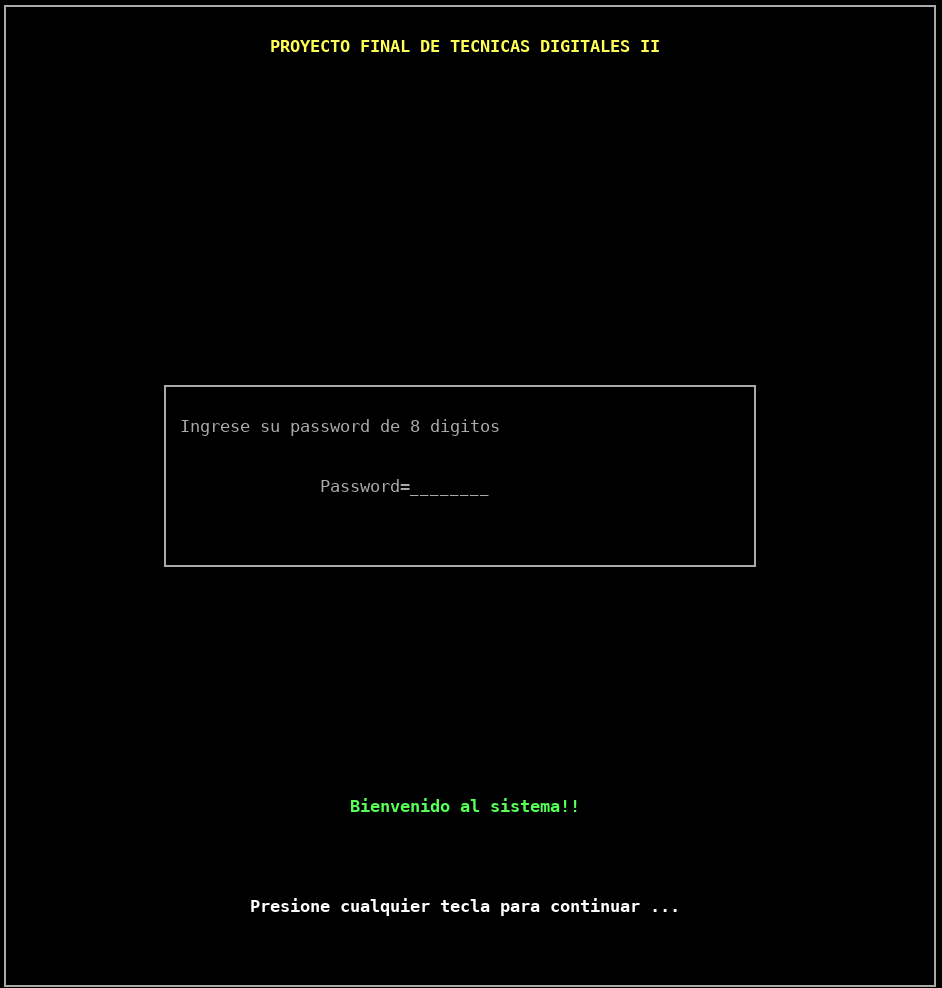
\includegraphics[width = 0.6\textwidth]{Imagenes/ingreso.png}
	\caption{Acceso al sistema.}
	\label{fig:pass}
\end{figure}

\subsection {Detección de tecla}
Se escribió una función análoga a $kbhit()$, que detecta si se presiono alguna tecla y retorna el valor tecleado.

\lstinputlisting[language=C, caption = deteccionTecla.c, label={list:deteccionTecla}]{code/deteccionTecla.c}

Uno de los aspectos fundamentales de esta parte del código es la función $no\_delay$, la cual hace que $getch()$ se transforme a una función no bloqueante, que devuelve un valor $ERR$ , predefinido en $nCurses$ si es que no se ha tipeado nada y devuelve el valor del carácter tipeado en caso contrario.

\subsection {Modo local y remoto}
Para pasar de un modo a otro basta con presionar la tecla \textbf{``R"}
\lstinputlisting[language=C, firstline=63 , lastline=80, caption =Fragmento de main.c ]{code/main.c}

\begin{figure}[H]
	\centering
	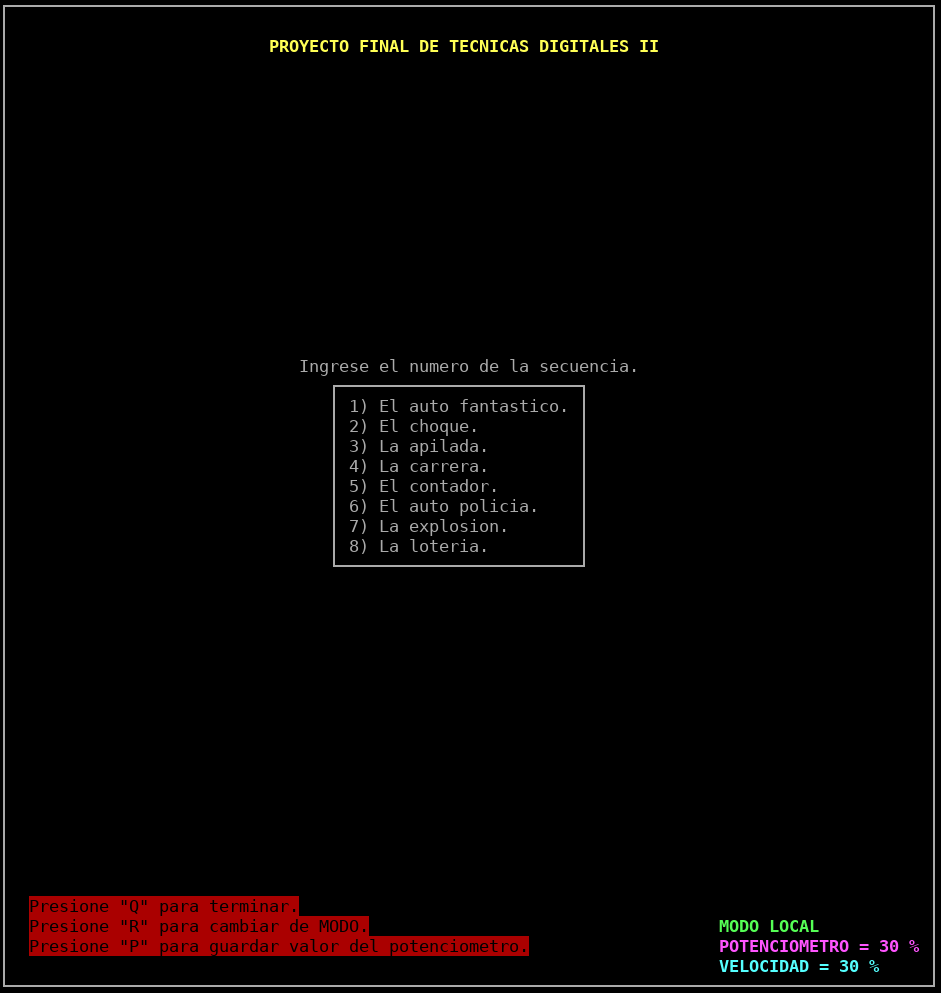
\includegraphics[width =0.5\columnwidth]{Imagenes/principal.png}
	\caption{Modo local.}
	\label{fig:local}
\end{figure}
\begin{figure}[H]
	\centering
	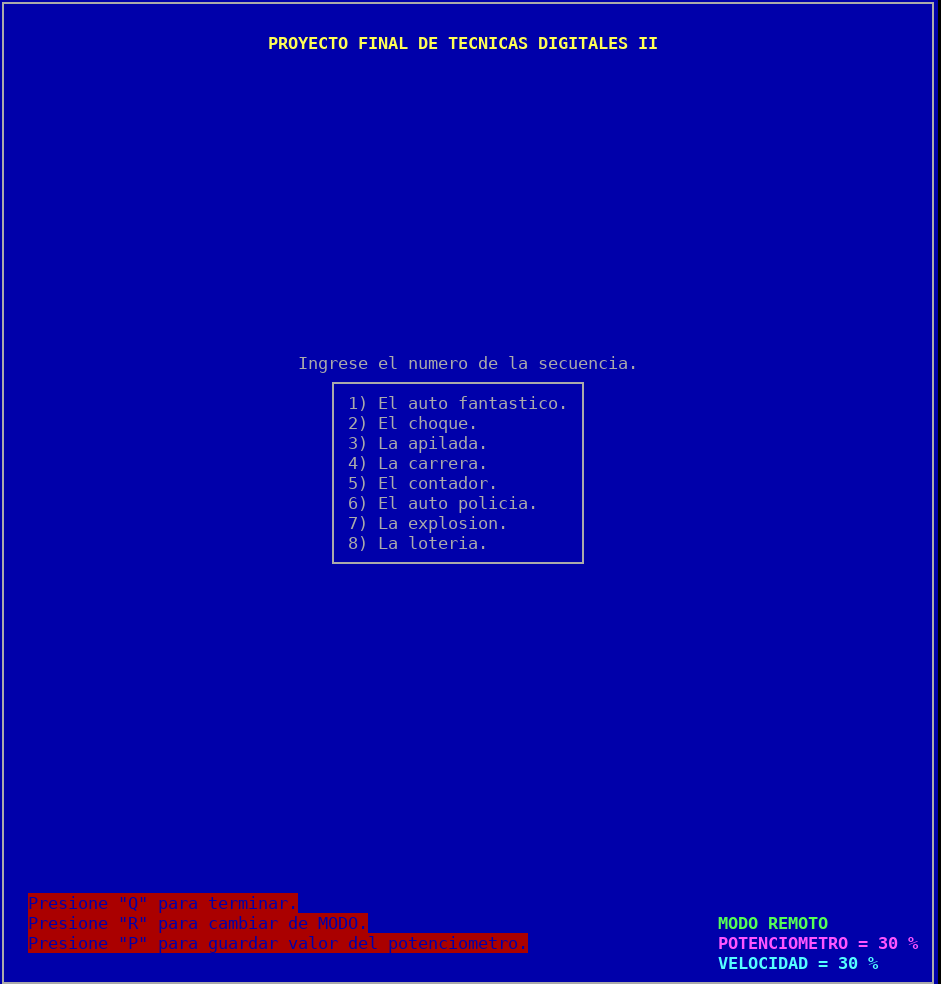
\includegraphics[width =0.5\columnwidth]{Imagenes/remoto.png}
	\caption{Modo remoto.}
	\label{fig:remoto}
\end{figure}
En cualquiera de los casos se modifica el valor de una variable bandera ``remoto", el cual determinar el color de la pantalla. Tanto los valores de remoto como potenciómetro y velocidad son pasados a la función $mainmenu()$ la cual se encarga de graficar el menú principal.

En el modo remoto los valores teclados se pasaran a la otra Raspberry (también configurada en modo remoto) a través de una comunicación serial.

\subsection {Secuencia}
Una vez seleccionada la secuencia se pasa a una pantalla similar donde se observa la secuencia ejecutándose y la velocidad de la misma, esta puede ser modificada a través de las flechas del teclado.

\lstinputlisting[language=C, caption = apilada.c, label={list:apilada.c}]{code/apilada.c}

Luego del algoritmo para la ejecución correcta de las luces, se comprueba si el programa debe ser remoto o local,en caso que sea remoto local, se pasan estos parámetros a los pines de salida, por el otro lado si fuese remoto se recibe el valor de la tecla presionada desde la otra terminal. 
\begin{figure}[H]
	\centering
	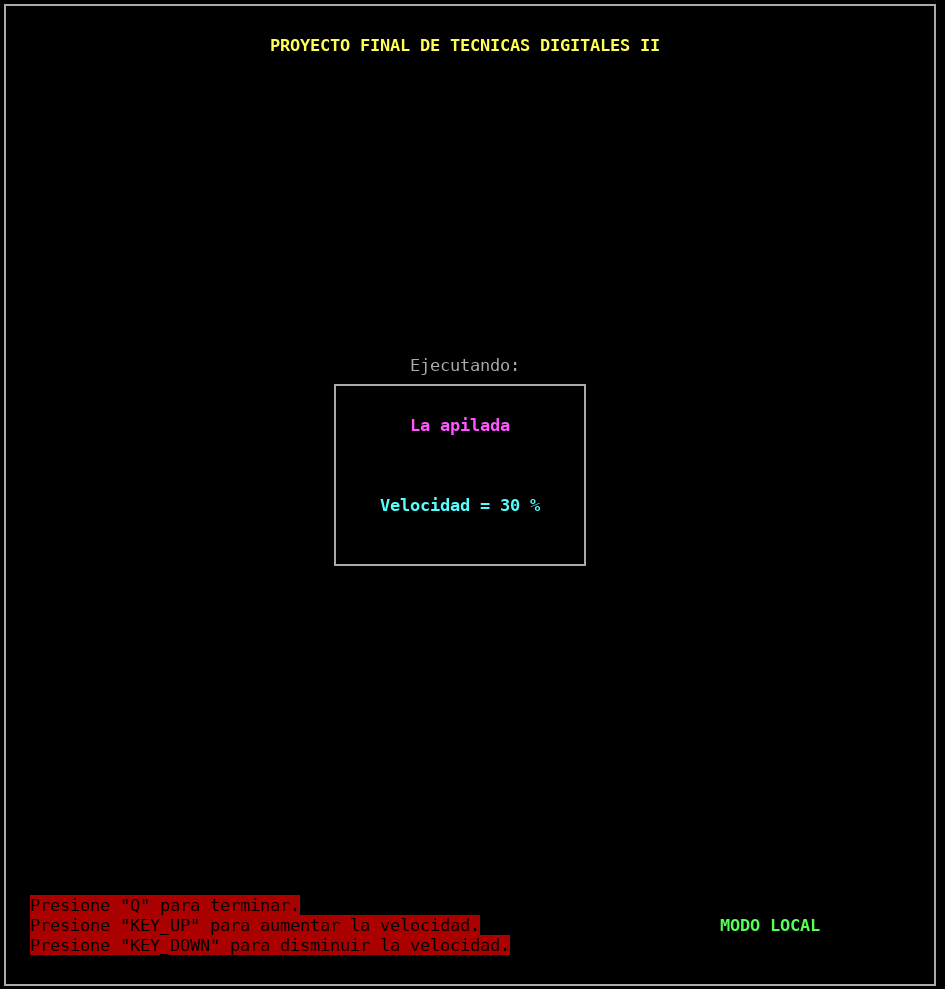
\includegraphics[width = 0.7 \columnwidth]{Imagenes/secuencia.png}
	\caption{Pantalla de una secuencia de luces.}
	\label{fig:secuencia}
\end{figure}

\section{Conclusión}
Para lograr el desarrollo del trabajo integrador, se requirió de los conocimientos y usos de los puertos de entrada y salida de la Raspberry Pi 3, utilización de librerías para el integrado pcf859, y protocolo de comunicación, tanto $I2C$ como serial entre dos puertos. 

A su vez crear encabezados y utilizar librerías que no habían sido necesarias para la primera presentación, con respecto al ordenador de placa reducida (Raspberry Pi 3), se observó y comprobó la versatilidad cuando se requiere velocidad y adaptación a otros terminales o periféricos.

En lo que respecta a conocimientos adquirido, se mejoró en la escritura de código, la fluidez a la hora de utilizar la terminal de software libre, los atajos, compilar, ejecutar y depurar con más eficiencia.
\end{document}

